\documentclass[12pt]{scrartcl}

\usepackage{tikz}
\usetikzlibrary{arrows}

\usepackage{amssymb}
\usepackage{amsmath}
\usepackage{algorithm}
\usepackage[noend]{algpseudocode}

\title{Compositional Safety Verification with Max-SMT}
\author{Fabian B\"{o}ller}
\date{\today}

\begin{document}

\maketitle

\section{Introduction}

This paper is based on the article `Compositional Safety Verification with Max-SMT` written by Marc Brockschmidt, Daniel Larraz, Albert Oliveras, Enric Rodrìguez-Carbonell and Albert Rubio.
They present an automated compositional program verification technique to verify safety properties for arbitrary programs.
In this paper we will inspect the inner workings of the algorithm with an example program which is minimal but at the same time covers all relevant parts of the algorithm.

\subsection{Compositional safety verification}

Safety verification in general is the task to ensure that an assertion at a certain program location is always true regardless of the input.
Formally a program is safe for an assertion if every evaluation path of the program leads to the fulfilment of the assertion.
While this description matches a global analysis, it is also possible to analyze components of a program and combine the results.
The advantage of this method is its scalability, but in many cases their is a loss in precision.

// TODO Why is it not trivial to do it compositional? (by example)

// Maybe put the explanation after the example program?

\subsection{Example program}

At this point I will present an example of a program graph, which will be as easy as possible but at the same point covers all necessary cases for everything following.
It will probably an example with three SCCs in a row, where the first has a transition to the second, the second has a transition to the third and the first has also a transition directly to the third.
This way there is an SCC with multiple entry transitions, which is crucial to show the tree-like exploration of SCCs.
There should be SCCs with just one node, but also more complex ones. The first to show the basic idea, the second to cover all parts of the algorithm.
The example should be an actual working program doing something useful, to enable understanding.

\begin{figure}
\centering
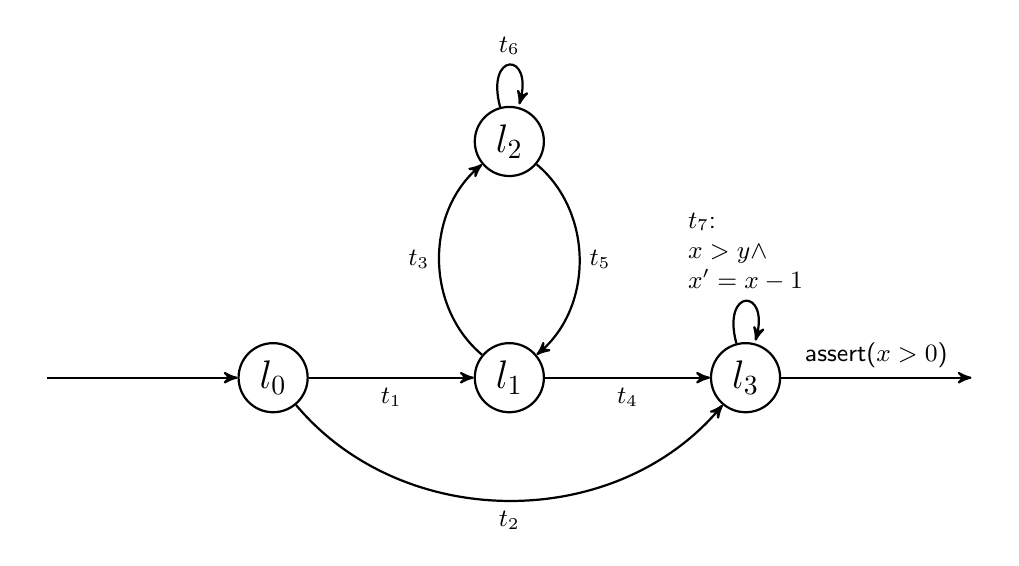
\begin{tikzpicture}[->,>=stealth',auto,node distance=3cm,
                    thick,main node/.style={circle,draw,font=\sffamily\Large\bfseries}]

  \node[main node] (0) {$l_0$};
  \node[main node] (1) [right of=0] {$l_1$};
  \node[main node] (2) [above of=1] {$l_2$};
  \node[main node] (3) [right of=1] {$l_3$};

  \node (4) [right of=3] {};
  \node (5) [left of=0] {};

  \path[every node/.style={font=\sffamily\small}]
    (0) edge node [below] {$t_1$} (1)
        edge [bend right=50] node [below] {$t_2$} (3)
    (1) edge [bend left=50] node [left] {$t_3$} (2)
        edge node [below] {$t_4$} (3)
    (2) edge [bend left=50] node [right] {$t_5$} (1)
        edge [loop above] node {$t_6$} (2)
    (3) edge [loop above] node [align=left] {$t_7$:\\$x > y \wedge$\\$x'= x - 1$} (3)
        edge node {assert($x>0$)} (4)
    (5) edge node {} (0);
\end{tikzpicture}
\caption{Example program}
\end{figure}

// TODO Construct example with: Simple SCC at the end as first example and Narrowing

\subsection{Definitions}

In this chapter we will introduce formal definitions for program graphs and invariants.

\subsubsection{Program}

We define $\mathcal{L} = \lbrace \ell_0, \dots, \ell_n \rbrace$ as the set of program locations, where $\ell_0$ denotes the unique start location of a program.
The example program uses the location set $\mathcal{L} = \lbrace \ell_0 , \ell_1 , \ell_2 , \ell_3 \rbrace$ and $\ell_0$ is its start location.
We define $\mathcal{V} = \lbrace v_1, \dots, v_n \rbrace$ as the set of variables which occur in a program.
An evaluation $\upsilon: \mathcal{V} \rightarrow \mathbb{Z}$ assigns each program variable an integer value.
A state $s = (\ell, \upsilon)$ represents the values of variables at a certain location $\ell \in \mathcal{L}$.
We denote with $\mathcal{F}(\mathcal{L})$ the set of formulas consisting of conjunctions of linear inequalities over the variables $\mathcal{V}$.
We define a program as a directed graph consisting of the program locations $\mathcal{L}$ and a set of transitions $\mathcal{T} = \lbrace (\ell, \tau, \ell') \mid \ell, \ell' \in \mathcal{L}, \tau \in \mathcal{F}(\mathcal{V} \cup \mathcal{V}') \rbrace$ between those locations.
An evaluation step with a transition $(\ell, \tau, \ell') \in \mathcal{T}$ leads a program state $(\ell, \upsilon)$ to another program state $(\ell', \upsilon')$ if and only if $\upsilon \models \tau$ and $\upsilon' \models \tau$. We then write $(\ell, \upsilon) \rightarrow_t (\ell', \upsilon')$.

We define a program component $\mathcal{C} \subseteq \mathcal{T}$ as a strongly connected component (SCC) of a program. 
We denote with $\mathcal{E}_\mathcal{C}$ its entry transitions which consists of all transitions $t = (\ell, \tau, \ell')$ such that $t \notin \mathcal{C}$ but $\ell'$ appears in $\mathcal{C}$.

We define an assertion as a pair $(t, \phi)$ where $t \in T$ and $\phi \in \mathcal{F}(\mathcal{V})$.
We say that a program is safe for an assertion if and only if $\forall (\ell_0, \upsilon_0): (\ell_0, \upsilon_0) \rightarrow_P^* \circ \rightarrow_t (\ell, \upsilon) \Rightarrow \upsilon \models \phi$.
We say that a program is conditional safe for an assertion if from a state where a precondition holds every path to an assertion also leads to the fulfilment of the assertion.

\subsubsection{Invariants}

An invariant is defined as an assignment $\mathcal{I} : \mathcal{L} \rightarrow \mathcal{F}(\mathcal{V})$ if and only if for all reachable states $(\ell, \upsilon)$ it holds that $\upsilon \models \mathcal{I}(\ell)$.

An invariant is an inductive invariant if and only if additionally it holds that $\top \models \mathcal{I}(\ell_0)$ and for all $(\ell, \tau, \ell') \in \mathcal{P}$ it holds that $\mathcal{I}(\ell) \wedge \tau \models \mathcal{I}(\ell')'$. We call the first initiation condition and the latter consecution condition.

An inductive invariant is an conditional inductive invariant if and only if for all $(\ell, \upsilon) \rightarrow_\mathcal{P} (\ell', \upsilon')$ it holds that $\upsilon \models \mathcal{Q}(\ell) \Rightarrow \upsilon' \models \mathcal{Q}(\ell')$.

For inductive invariants I will show additionally the possible construction directions top-down and bottom-up.

\subsection{Algorithm by example}

The idea is to explain it the other way around than in the paper.
This way I can cover the whole picture and then dive into detail.
The explanation will be done by the presented example.

\subsubsection{CheckSafe}

Here we will view the SCCs as components and abstract from the details of CondSafe.

Basic Algorithm:

\begin{enumerate}
  \item Begin at the end to reach the initial states in a tree which is to discover
  \item We must descend the tree to all of the initial states to prove safety
  \item If we can not descend further in a path of the tree, find other conditions (narrow)
\end{enumerate}

\subsubsection{CondSafe}

Here we will inspect the different SCCs and apply CondSafe to them

\subsection{Definition of the algorithm}

At this point we will present the formal algorithms for CheckSafe and CondSafe.
Since CondSafe is based on Max-SMT-Solving, we will first introduce this extension of an SMT-Solver.

\subsubsection{Max-SMT}

Let $\mathcal{P}$ be a fixed set of propositional variables.
We call $p$ and $\neg p$ literals for all $p \in \mathcal{P}$.
We define a clause as disjunction of literals $l_1 \vee \dots \vee \l_n$ and a propositional formula as conjunction of clauses $C_1 \wedge \dots \wedge C_m$.

With a SAT-Solver it is possible to determine if a propositional formula is satisfiable.
An SMT-Solver is able to check the satisfiablity of a formula with literals from a given background theory.
For both solvers there exist extensions called Max-SAT and Max-SMT.
Those extensions provide the possibility to declare constraints as soft with a weight.
A soft constraints does not have to be satisfied, but the solver will try to maximize the sum of the weights of the soft constraints.

Formally a Max-SMT problem is a formula $H_1 \wedge \dots \wedge H_n \wedge [S_1,\omega_1] \wedge \dots \wedge [S_m,\omega_m]$, where $H_i$ denote the hard clauses, which also occur in an SMT problem, and $[S_i,\omega_i]$ denote the soft clauses and their weight.

To find conditional inductive invariants for program parts we create hard constraints for the consecution and safety conditions and a soft constraint for the initiation condition.
While the consecution condition ensures that the invariant is inductive and the safety condition ensures the assertion is implied, the initiation condition does not need to be fulfiled and thus the resulting invariant might depend on additional preconditions.  

In the definition of the condition we use the template \[ I_{\ell,k}(\mathcal{V}) \equiv \bigwedge_{1 \leq j \leq k}{I_{\ell,j,k}(\mathcal{V})} \] which is a conjunction of $k$ linear inequations \[ I_{\ell,j,k}(\mathcal{V}) \equiv i_{\ell,j} + \sum_{v \in \mathcal{V}}{i_{\ell,j,v} * v} \leq 0 \]. We write $I'_{\ell,k}$ instead of $I_{\ell,k}$ if we use variables $i'_{l,j}$ and $i'_{l,j,v}$ instead of $i_{l,j}$ and $i_{l,j,v}$.
With those definitions we define the initiation condition for a transition $t = (\ell, \tau, \ell') \in \mathcal{E}_\mathcal{C}$ and numbers $j, k \in \mathbb{N}$ with $1 \leq j \leq k$ as \[ \mathbb{I}_{t,j,k} \equiv \tau \Rightarrow I'_{l',j,k} \]. For each transition $t = (\ell, \tau, \ell') \in \mathcal{C}$ and number $k \in \mathbb{N}$ we define the consecution condition as \[ \mathbb{C}_{t,k} \equiv I_{\ell,k} \wedge \tau \Rightarrow I'_{\ell,k} \]. The safety condition we define for an exit transition $t_\text{exit} = (\tilde{\ell}_\text{exit}, \tau_\text{exit}, \ell_\text{exit})$ as \[ \mathbb{S}_k \equiv I_{\tilde{\ell}_\text{exit},k} \wedge \tau_\text{exit} \Rightarrow \varphi' \].

Those templates for the three different conditions we can put together in a Max-SMT problem:
\[ \mathbb{F}_k \equiv \bigwedge_{t \in \mathcal{C}} \mathbb{C}_{t, k} \wedge \bigwedge_{t \in \mathcal{E}_\mathcal{C}, 1 \leq j \leq k}{(\mathbb{I}_{t,j,k} \vee \neg p_{\mathbb{I}_{t,j,k}})} \wedge \mathbb{S}_k \wedge \bigwedge_{t \in \mathcal{E}_\mathcal{C}, 1 \leq j \leq k}{[p_{\mathbb{I}_{t,j,k}}, \omega_\mathbb{I}]} \]

\subsubsection{CheckSafe}

\begin{algorithm}
\caption{CheckSafe}\label{checksafe}
\begin{algorithmic}[1]
\State $\mathcal{P} \gets \text{program}$
\State $\mathcal{C} \gets \text{strongly connected component}$
\State $\mathcal{E}_\mathcal{C} \gets \text{entry transitions of } \mathcal{C}$
\State $(t_\text{exit}, \varphi) \gets \text{assertion with exit transition } t_\text{exit} \text{ and clause } \varphi$
\State $(\ell_\text{exit}, \tau_\text{exit}, \ell'_\text{exit}) \gets t_\text{exit}$
\If {$\tau_\text{exit} \Rightarrow \varphi'$}
  \Return Safe
\ElsIf {$\ell_\text{exit} = \ell_0$}
  \Return Maybe
\EndIf
\State $\mathcal{Q} \rightarrow \text{CondSafe}(\mathcal{C}, \mathcal{E}_\mathcal{C}, (t_\text{exit}, \varphi))$
\If {$\mathcal{Q} = \text{None}$}
  \Return Maybe
\EndIf
\ForAll {$t = (\ell, \tau, \ell') \in \mathcal{E}_\mathcal{C}, \mathcal{L} \in \mathcal{Q}(\ell')$}
  \State $\tilde{\mathcal{C}} \gets \text{component}(\ell, \mathcal{P})$
  \State $\mathcal{E}_{\tilde{\mathcal{C}}} \gets \text{entries}(\tilde{\mathcal{C}}, \mathcal{P})$
  \State $\text{res}[t, \mathcal{L}] \gets \text{CheckSafe}(\mathcal{P}, \tilde{\mathcal{C}}, \mathcal{E}_{\tilde{\mathcal{C}}}, (t, \mathcal{L}))$
\EndFor
\If {$\forall t = (\ell, \tau, \ell') \in \mathcal{E}_\mathcal{C}, \mathcal{L} \in \mathcal{Q}(\ell'): \text{res}[t, \mathcal{L}] = \text{Safe}$}
  \Return Safe
\Else
  \State $\tilde{\mathcal{E}}_{\tilde{\mathcal{C}}} \gets \lbrace (\ell, \tau \wedge \neg (\bigwedge_{\mathcal{L} \in \mathcal{Q}(\ell') \wedge \text{res}[t, \mathcal{L}]=\text{Maybe}}{\mathcal{L}'}), \ell') \mid t = (\ell, \tau, \ell') \in \mathcal{E}_\mathcal{C} \rbrace$
  \State $\tilde{\mathcal{C}} \gets \lbrace (\ell, \tau \wedge \neg\mathcal{Q}(\ell')' \wedge \neg\mathcal{Q}(\ell), \ell') \mid (\ell, \tau, \ell') \in \mathcal{C} \rbrace$
\EndIf
\Return $\text{CheckSafe}(\mathcal{P}, \tilde{\mathcal{C}}, \tilde{\mathcal{E}}_{\tilde{\mathcal{C}}}, (t_\text{exit}, \varphi))$
\end{algorithmic}
\end{algorithm}

\subsubsection{CondSafe}

\begin{algorithm}
\caption{CondSafe}\label{condsafe}
\begin{algorithmic}[1]
\State $\mathcal{C} \gets \text{strongly connected component}$
\State $\mathcal{E}_\mathcal{C} \gets \text{entry transitions of } \mathcal{C}$
\State $(t_\text{exit}, \varphi) \gets \text{assertion with exit transition } t_\text{exit} \text{ and clause } \varphi$
\State $k \gets 1$
\Repeat
  \State construct formula $\mathbb{F}_k$ from $\mathcal{C}$, $\mathcal{E}_\mathcal{C}$ and $t_\text{exit}, \varphi$
  \State $\sigma \gets \text{MAX-SMT-Solver}(\mathbb{F}_k)$
  \If {$\sigma$ is a model}
    \State $\mathcal{Q} \gets \lbrace \ell \rightarrow \sigma(I_{\ell, k}) \mid \ell \in \mathcal{C} \rbrace$
    \Return $\mathcal{Q}$
  \EndIf
  \State $k \gets k + 1$
\Until{$k > \text{MAX\_CONJUNCTS}$}
\Return None
\end{algorithmic}
\end{algorithm}

// TODO At this point I will link the presented example to the algorithm code and give the definition of the algorithms.

\end{document}
